\chapter{Empirical Analysis}\label{empirical}
\section{Overview}\label{expoverview}
To evaluate Polyanya OkNN we consider two distinct setups and one large map with 
containing 9000 polygonal obstacles (this benchmark is described further in the next section).

In the first setup, targets are numerous and densely distributed throughout
the map. Our principal point of comparison in this case is \textit{LVG}~\cite{zhang2004spatial} which
is a state of the art method based on incremental visibility graphs. 
In the second setup, targets are few and sparsely distributed.
Our principal point of comparison in this case is \textit{brute-force Polyany}.
We motivate these decisions as follows:

\begin{itemize}[leftmargin=1cm]
\item When the map is large and targets are many (commonly the case in spatial database settings) \textit{LVG} considers only a small part of map and so its query processing can be very fast.
  \textit{Brute-force Polyany} meanwhile is infeasible to run (there are too many searches).

\item When the map is large targets are few ($<=10$) \textit{LVG} builds a visibility graph for almost entire map,
  and ends up with quadratic runtime complexity, which is unacceptable.
    Meanwhile, brute force \textit{Polyanya}, which is a very fast point-to-point pathfinding algorithm,
    can be competitive even when called repeatedly.
    This comparison is motivated by recent prior work involving kNN queries on road networks~\cite{abeywickrama2016k},
    where other fast point-to-point algorithms were shown to provide state-of-the-art performance in multi-targets scenarios,
    even when compared against dedicated kNN algorithms.
\end{itemize}

In experiments, we examine performance based on elapsed time and expanded search node.
For \textit{LVG}, we count the number of expanded node in \textit{Dijkstra}.

The navigation mesh of map is generated by \textit{Constrained Delaunay Triangulation}, which is $O(nlogn)$;
the implementation of such algorithm is in library \textit{Fade2D} \footnote{http://www.geom.at/fade2d/html},
the total time on such preprocessing is about 6s.
We implemented in C++ the LVG algorithm (more details below) as well as two versions of multi-target Polyanya:
one each for Target and Interval Heuristic.
Our code is compiled with \textit{clang-902.0.39.1} using \textit{-O3} flag,
under \textit{x86\_64-apple-darwin17.5.0} platform.
All of our source code and test data set are  publicly available \footnote{http://bitbucket.org/dharabor/pathfinding}
All experiments are performed on a 2.5 GHz Intel Core i7 machine with 16GB of RAM and running OSX 10.13.4. 


\section{Implementation of \textit{LVG}}\label{imptlvg}
As discussed \textit{LVG} is our primary competitor in experiments with dense targets.
However, since there is no publicly available implementation, we write one ourselves.
We implement the method as per the description in the original paper~\cite{zhang2004spatial}.
The only differences is in construction of the visibility graph:
\textit{LVG} uses the rotational plane-sweeping algorithm from~\cite{sharir1986shortest} which runs worst case $O(n^2logn)$ time.
In our work we opted to simplify development complexity and use a $R^*$-tree\cite{beckmann1990r} query for visibility checking.
Each such query runs in $log(n)$ time  and we perform one check for each unique pair of vertices.
Thus the total complexity to build a visibility graph is also $O(n^2logn)$.
This implementation, as with the rest of our code, is made publicly available.

The implmentation of $R^*$-tree we use is also publicly available \footnote{https://github.com/safarisoul/ResearchProjects/tree/master/2016-ICDE-RkFN},
and appears in other recently published work~\cite{wang2016efficiently}.

\section{Benchmark}\label{dataset}

\begin{figure*}[!hbt]
  \centering
  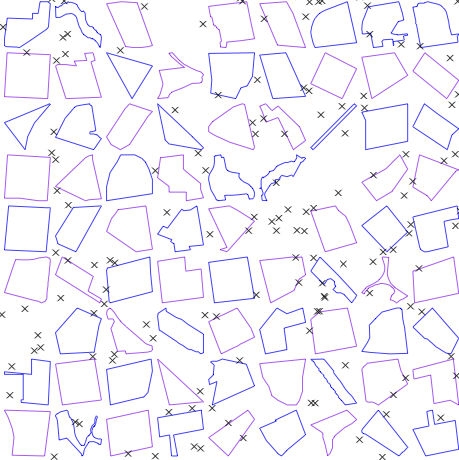
\includegraphics[width=.7\linewidth]{pic/distribution.png}
  \caption{\small Example: a generated map with many targets. Color border polygons are
  obstacles, black crosses are targets.}\label{distribution}
\end{figure*}

The data set from our main competitor LVG\cite{zhang2004spatial}
is no longer available on the public Internet so we opt to generate new benchmark problems.
We extract the shape of all parks in Australia from \textit{OpenStreetMap}\cite{OpenStreetMap} and
use these shapes as polygonal obstacles. There are about 9000 such polygons in total.
Next we generate a map by tiling all obstacles in the empty square plane.
For the tiling, we first divide the square plane into grid having $\lceil\sqrt{|O|}\rceil$ number of rows and columns.
Then we assign each polygon to a single grid cell and normalize the shape of polygon by to fit inside the cell.
Figure~\ref{distribution} gives an example a map generated in this way.
For each experiment, we're using $1000$ random query points, grouping results by
\textit{x-axis}, and computing average; the size of each bucket is at least 10. 

One thing needs to be highlighted is that,
unlike \textit{LVG} ~\cite{zhang2004spatial} where obstacles are always rectangular,
we consider polygons of arbitrary shape, which is more realistic and potentially more challenging as there are more vertices to consider.
The total number of vertices across all polygons is more than 100,000. 

\section{Experiment 1: lower bounds on performance}\label{exp1}
\begin{figure*}[!htb]
  \begin{subfigure}{\linewidth}
    \begin{subfigure}{0.5\textwidth}
        \centering
        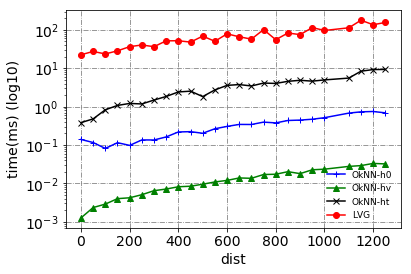
\includegraphics[width=.9\textwidth]{pic/e1_dense_time.png}
        \caption{}
        \label{e1_dense_time}
    \end{subfigure}%
    \hfill
    \begin{subfigure}{0.5\textwidth}
        \centering
        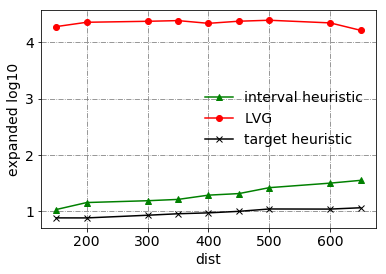
\includegraphics[width=.9\textwidth]{pic/e1_dense_gen.png}
        \caption{}
        \label{e1_dense_gen}
    \end{subfigure}
    \caption*{\small Dense experiment: $|T| \approx |O|,k=1$}
  \end{subfigure}\par\medskip
  \begin{subfigure}{\linewidth}
    \begin{subfigure}{0.5\textwidth}
        \centering
        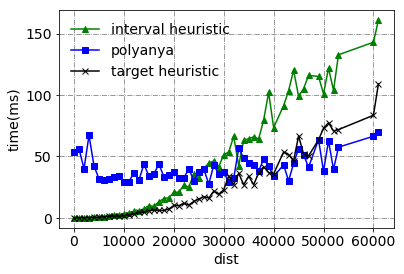
\includegraphics[width=.9\textwidth]{pic/e1_sparse_time.png}
        \caption{}
        \label{e1_sparse_time}
    \end{subfigure}%
    \hfill
    \begin{subfigure}{0.5\textwidth}
        \centering
        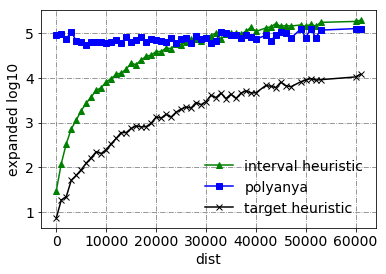
\includegraphics[width=.9\textwidth]{pic/e1_sparse_gen.png}
        \caption{}
        \label{e1_sparse_gen}
    \end{subfigure}
    \caption*{\small Sparse experiment: $|T| = 5, k=1$}
  \end{subfigure}
  \caption{\small Experiment1: examine the performance when $dist$ increase, where
  $dist$ is the obstacle distance to retrieved target}
\end{figure*}

This experiment aims to examine the performance of proposed algorithms in the easiest case, which is $k=1$.
Results show that in dense targets scenario, the proposed algorithms outperform \textit{LVG} in both space and time (fig~\ref{e1_dense_time},\ref{e1_dense_gen}).

In the sparse targets scenario, \textit{target heuristic} has the smallest number of node
operations (fig~\ref{e1_sparse_gen}), 
and both \textit{target} and \textit{interval} heuristic are outperformed on runtime by brute-force \textit{Polyanya} (fig~\ref{e1_sparse_time}) as $dist$ increases.
These results suggest the \textit{interval heuristic} has a large search space, and the
\textit{target heuristic} has a costly heuristic function. Results also show that \textit{brute-force Polyanya} is
not sensitive to $dist$, the reason is that it has to run a point-to-point search to all
targets no matter where the nearest neighbor is. 

\section{Experiment 2: computing more nearest neighbor}\label{exp2}
\begin{figure*}[!htb]
  \begin{subfigure}{\linewidth}
    \begin{subfigure}{0.5\textwidth}
        \centering
        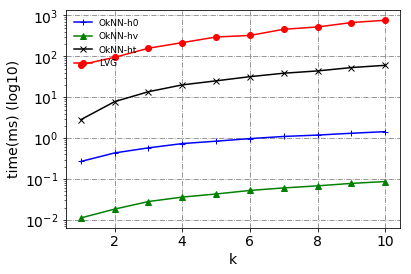
\includegraphics[width=.9\textwidth]{pic/e2_dense_time.png}
        \caption{}
        \label{e2_dense_time}
    \end{subfigure}%
    \hfill
    \begin{subfigure}{0.5\textwidth}
        \centering
        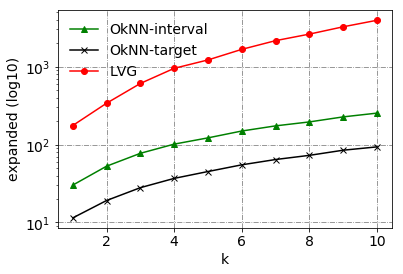
\includegraphics[width=.9\textwidth]{pic/e2_dense_gen.png}
        \caption{}
        \label{e2_dense_gen}
    \end{subfigure}
    \caption*{\small Dense: $k \in [1,...10], |T| \approx |O|$}
  \end{subfigure}\par\medskip
  \begin{subfigure}{\linewidth}
    \begin{subfigure}{0.5\textwidth}
        \centering
        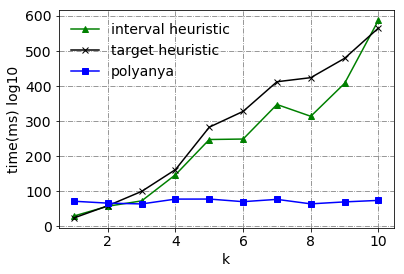
\includegraphics[width=.9\textwidth]{pic/e2_sparse_time.png}
        \caption{}
        \label{e2_sparse_time}
    \end{subfigure}%
    \hfill
    \begin{subfigure}{0.5\textwidth}
        \centering
        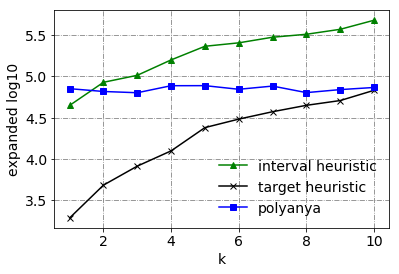
\includegraphics[width=.9\textwidth]{pic/e2_sparse_gen.png}
        \caption{}
        \label{e2_sparse_gen}
    \end{subfigure}
    \caption*{Sparse: $k \in [1,...10], |T|=10$}
  \end{subfigure}
  \caption{\small Experiment2: examine the performance when $k$ increase}
\end{figure*}
%
This experiment aims to examine the performance of algorithm when query becomes harder ($k$ increasing).
Results show that, in the dense targets scenario, the proposed algorithms still outpeform \textit{LVG}, even as $k$ increases (fig~\ref{e2_dense_time},\ref{e2_dense_gen}).
In the sparse targets scenario, results show that brute-force $Polyanya$ is not sensitive to $k$.
Meanwhile each of the two OkNN variants requires increasing amounts of node operations (and thus memory) and become quickly outperformed.
A side effect of \textit{target heuristic} when $k$ increase is that \textit{lazy reassign} causes extra node expansions.

\section{Experiment 3: changing number of targets}\label{exp3}

\begin{figure*}[!htb]
    \centering
    \begin{subfigure}{0.5\textwidth}
        \centering
        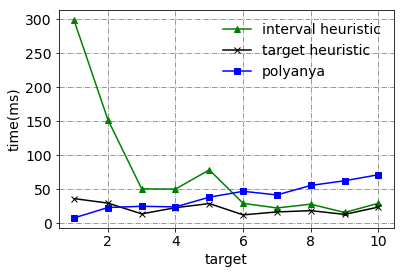
\includegraphics[width=.9\textwidth]{pic/e3_time.png}
        \caption{}
        \label{e3_time}
    \end{subfigure}%
    \hfill
    \begin{subfigure}{0.5\textwidth}
        \centering
        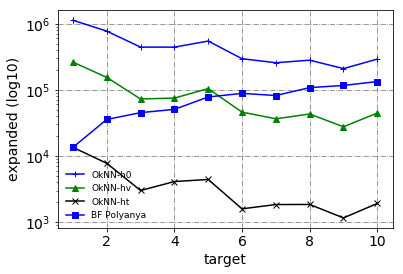
\includegraphics[width=.9\textwidth]{pic/e3_gen.png}
        \caption{}
        \label{e3_gen}
    \end{subfigure}
    \caption{\small Experiment 3: examine the performance when $|T|$ increase, $k=1, |T| \in [1,...10]$}
\end{figure*}

This experiment is run only on the sparse target set. It aims to examine the scalability of the proposed algorithms with an increasing
(but still sparse) number of targets.

Results show that proposed algorithms gradually outperform brute force \textit{Polyanya} in both time and node operations (fig~\ref{e3_time},\ref{e3_gen}).
This implies that the proposed OkNN variants algorithms are much better choices when the set of targets increase. 
Also notice that the node expansion decreases when $|T|$ goes large,
for \textit{interval heuristic}, the reason is that search nodes can reach target earlier; for
\textit{target heuristic}, in addition to previous reason, the \textit{R-tree} query in
heuristic function has good scalability. 
Although we have seen in other experiements that brute-force \textit{Polyanya} has an advantage when $k$ is large, this advantaged disappears as $|T|$ grows.
In some practical settings $|T|$ can be in the hundreds or thousands, e.g.~\cite{abeywickrama2016k} while $k$ is usually orders of magnitude smaller. 

\section{Experiment 4: behavior of target heuristic}\label{exp4}
From previous experiments, we notice that the \textit{target heuristic} always has smaller search space,
but it's sometimes orders of magnitudes slower than other competitors.
Thus, we want to dig out more details about the behavior of $h_t$.
This experiment aims to examine the target heuristic from following aspects:
\begin{itemize}
  \item the ratio of the cost on the heuristic function in total elapsed time;
  \item the ratio of the reassignment in total expanded nodes;
  \item the ratio of the heuristic function call in total expanded nodes;
\end{itemize}.

\subsection{Ratio of heuristic cost}
Figure~\ref{hcost} shows the distribution of ratio:
$\textit{heuristic cost} / \textit{total cost}$.
\begin{figure}[htp]
  \centering
  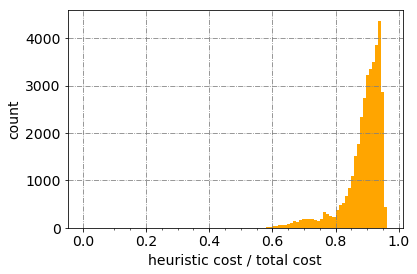
\includegraphics[width=.7\linewidth]{./pic/hcost.png}
  \caption{\small Records from experiments 1,2,3 produce the plot}
  \label{hcost}
\end{figure}
The result shows that the $h_t$ cost $\approx 90\%$ of total time, meaning that
\textit{target heuristic} needs at least an order of magnitude smaller search space 
to outperform competitors.

\subsection{Side effect}
Figure~\ref{lazy_reassign} shows the ratio of \textit{lazy reassignment} when $k$ increase.
\begin{figure}[htp]
  \centering
  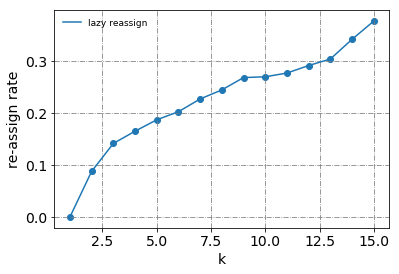
\includegraphics[width=.7\linewidth]{./pic/lazy_reassign.png}
  \caption{\small Records from experiments 1,2,3 produce the plot.}
  \label{lazy_reassign}
\end{figure}
The result shows that the side effect-\textit{reassignment} happens more freqently when $k$
increase, meaning that \textit{target heuristic} is more suitable for small $k$.

\subsection{Ratio of heuristic call}
Figure~\ref{lazy_compute} shows the distribution of ratio:
$\textit{heuristic call} / \textit{expanded nodes}$.
\begin{figure}[htp]
  \centering
  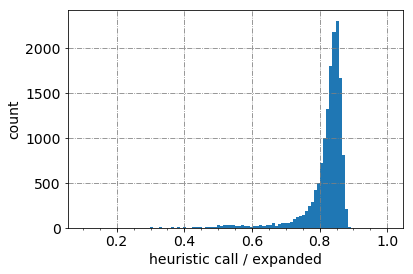
\includegraphics[width=.7\linewidth]{./pic/lazy_compute.png}
  \caption{\small Records from experiments 1,2,3 where $k=1$ produce the plot.}
  \label{lazy_compute}
\end{figure}
To ignore the side effect when $k>1$, this plot only considers those records with $k=1$.
The plot implies the effect of \textit{lazy compute} can reduce $\approx 15\%$ heuristic call in
the search.

\section{Summary}
This chapter is to evaluate proposed algorithms.
In the chapter, we've discussed the motivation of experiment design,
the benchmark problem, and results of the experiment.
From these experiements, we can see that proposed algorithms outpeform the state-of-the-art
orders of magnitudes, and between these proposed algorithms, they have different suitable
scenarios.
